\documentclass[a4paper,10pt]{report}
\usepackage[utf8x]{inputenc}
\usepackage{graphicx}

%opening
\title{Trainmining}
\author{}


\begin{document}
\newcommand\litem[1]{\item{\bfseries #1 }}
\renewcommand{\abstractname}{Executive Summary}
\begin{abstract}

\end{abstract}


\maketitle
\setcounter{chapter}{1}
\chapter{Data analysis}
\section{Alarm database}
The alarm database has is structured as follows:\cite{Feyyad1996}
\subsubsection*{Table ER\_ERRORS}
Contains every alarm received by the Maintenance Station. Has the following fields:
\begin{itemize}
 \item DVNI\_ERRORNUMBER - Alarm identifier
 \item DVNS\_ERRORTIME - Time-stamp for the alarm
 \item DVNI\_INSTALLATIONCODE - Code of the installation in which the alarm was raised
 \item DVNI\_SENDERINSTALLATIONCODE - Code of the installation from which the alarm was sent (might be different from the one which raised it)
\end{itemize}

\subsubsection*{Table IG\_INSTALLATIONGENERAL}
This table contains information on all the installations. Has the following fields:
\begin{itemize}
 \item DVNI\_INSTALLATIONCODE - Installation identifier
 \item DVNI\_SYSTEMCODE - Type of system, as defined in the ``SG\_SYSTEMSGENERAL'' table
 \item DVNI\_VERSION - System version
 \item DVAC\_SHORTNAME - Short name of the installation
 \item DVAC\_INSTALLATIONNAME - Name of the installation
 \item DVAC\_LOCATION - Location for the installation
 \item CHK\_IS\_NODE - Whether it is a node (doesn't directly send alarms, only raise them) or not
\end{itemize}

\subsubsection*{Table IG\_NODO\_INSTALLATION}
This table gathers additional information on installations which are nodes. This is, installations that can raise alarms but need a Parent installation to send them. Has the following fields:
\begin{itemize}
 \item IG\_NODO\_INSTALLATION - Identifier of the installation which is a node
 \item DVNI\_FATHER\_INSTALLATION - Identifier of the parent installation
\end{itemize}

\subsubsection*{Alarm information tables ERH\_ERRORS\_HSL1 or ERS\_ERRORS\_SAM\_ENCE}
Both these tables record information on the alarms. Either one or other table is filled depending on which version of the system is installed in the station. However, in terms of information, both contain the following fields:
\begin{itemize}
 \item DVNI\_ERRORNUMBER - Alarm identifier
 \item MESSAGE\_ID - Unique alarm identifier
 \item MESSAGE\_TYPE - Type of alarm, always set as ``notification'' (not relevant)
 \item INVOKE\_TYPE - Tells whether the alarm has generated itself due to a connection or disconnection (if type is ``node'') or is generated by a diagnosis system (``saml'') or energy system (``energy'')
 \item INVOKE\_NAME - Irrelevant, always set to ``diagnosis''
 \item EVENT\_TYPE - Defines the type of alarm which has been generated. Its possible values will be described afterwards.
 \item ADDITIONAL\_TEXT - Alarm code
 \item ADDITIONAL\_INFOS - Additional parameters to be shown in error message
 \item DVNI\_ERRORCATEGORY - Alarm severity. Values from 1 to 5 indicating importance of the alarm, or -1 if the alarm indicates recovery from a previous failure.
\end{itemize}
The ``ERH\_ERRORS\_HSL1'' table, has one additional field:
\begin{itemize}
 \item CLAZZ - Shows the type of system which has sent the alarm
\end{itemize}
The field ``EVENT\_TYPE'' can have one of the following values:
\begin{itemize}
  \item fieldElementAlarm - Alarm related to a field element
  \item fieldElementFailure - Failure in a field element
  \item operatorInformation - Information to the operator
  \item imCpuAndCommunications - Related to IM CPU or IM communications
  \item internalDiagnosis - Internal diagnosis of a system
  \item operationsDiagnosisCommunications - Communication error in Operation and Diagnosis systems
  \item ImFecVersions - IM or FEC version
  \item internalTraces - Internal traces of a system
  \item operatorCommandAnswer - Answer to an operator command
  \item CommProblem - Undefined communication problem
  \item Information - Information message: versions, etc.
  \item CommunicationsAlarm - Procedures and processes to carry information from one point to other
  \item QualityOfServiceAlarm - Loss of quality of service
  \item ProcessingErrorAlarm - SW or processing error
  \item EquipmentAlarm - Equipment failure
  \item EnvironmentAlarm - Related to the environment where the system is located
  \item other - Other
\end{itemize}

\section{Statistic analysis}
\subsection{Alarm classification}
In order to have a better insight of the provided databases and the mentioned descriptions, a preliminary insight was made, quantitatively analysing some of the parameters which seemed more relevant for alarm definition. Specifically, the chosen parameters are the following:

\begin{itemize}
 \item EVENT\_TYPE
 \item INVOKE\_TYPE
 \item DVNI\_ERRORCATEGORY (Error Category)
\end{itemize}

The proportion of each kind of alarms in each of the provided databases (Antequera, Camas, Segovia and Sevilla) is as follows:
\begin{figure}[ht!]
 \centering
 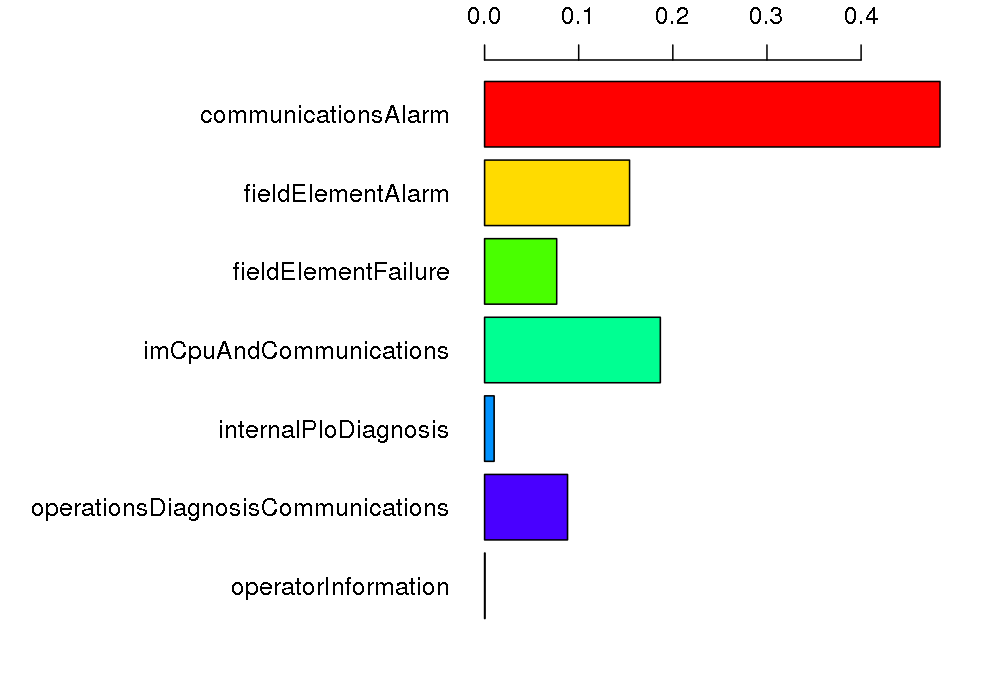
\includegraphics[width=\textwidth]{./img/antequera_graph.png}
 \caption{Alarm information for Antequera}
 \label{fig:anteq}
\end{figure}
\begin{figure}[ht!]
 \centering
 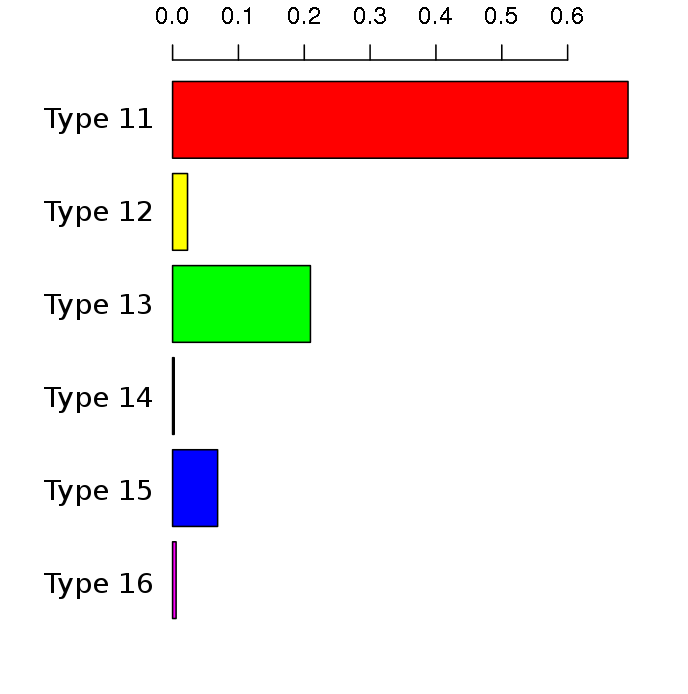
\includegraphics[width=\textwidth]{./img/segovia_graph.png}
 \caption{Alarm information for Segovia}
 \label{fig:segovia}
\end{figure}
\begin{figure}[ht!]
 \centering
 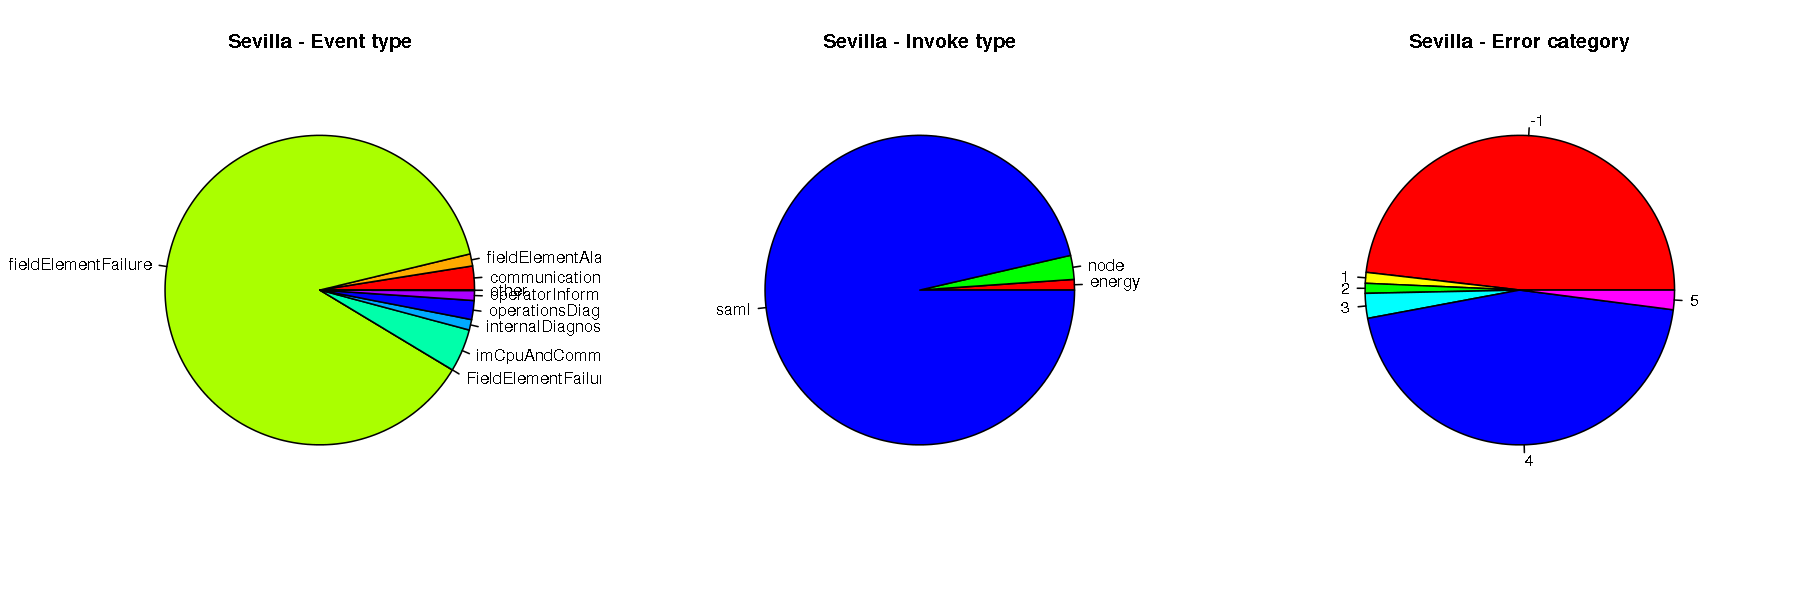
\includegraphics[width=\textwidth]{./img/sevilla_graph.png}
 \caption{Alarm information for Sevilla}
 \label{fig:sevilla}
\end{figure}

In Sevilla, we observe an additional error category marked as ``other''. If we make a deeper insight on those errors, we find that is a group formed by 77 alarms of the same type.

\subsubsection{Hourly timeline}

In order to make a first approach to data analysis, we decided to analyse the alarms on a hourly distribution, checking which types of alarms are more likely to happen in different hours during the day. The result is the following:

\clearpage

\begin{figure}[h!]
 \centering
 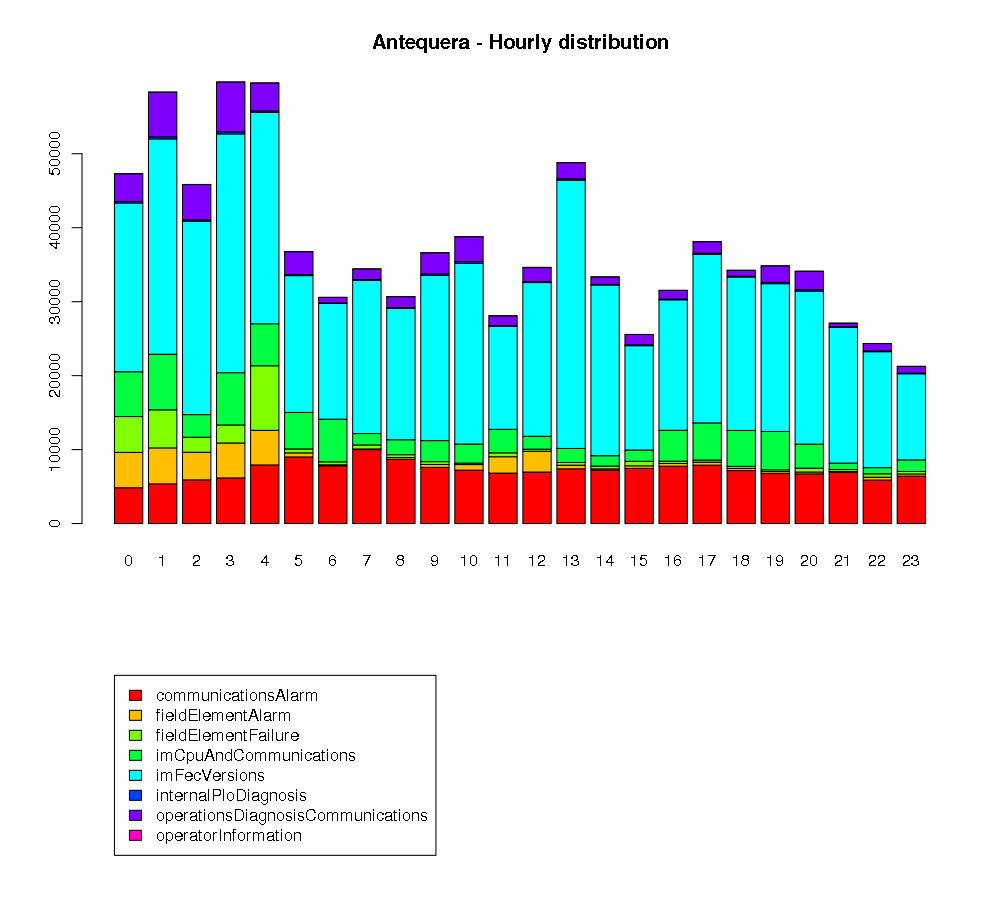
\includegraphics[height=0.4\textheight]{./img/antequera_timeline.png}
 \caption{Hourly distribution for Antequera (stacked)}
\end{figure}
\begin{figure}[h!]
 \centering
 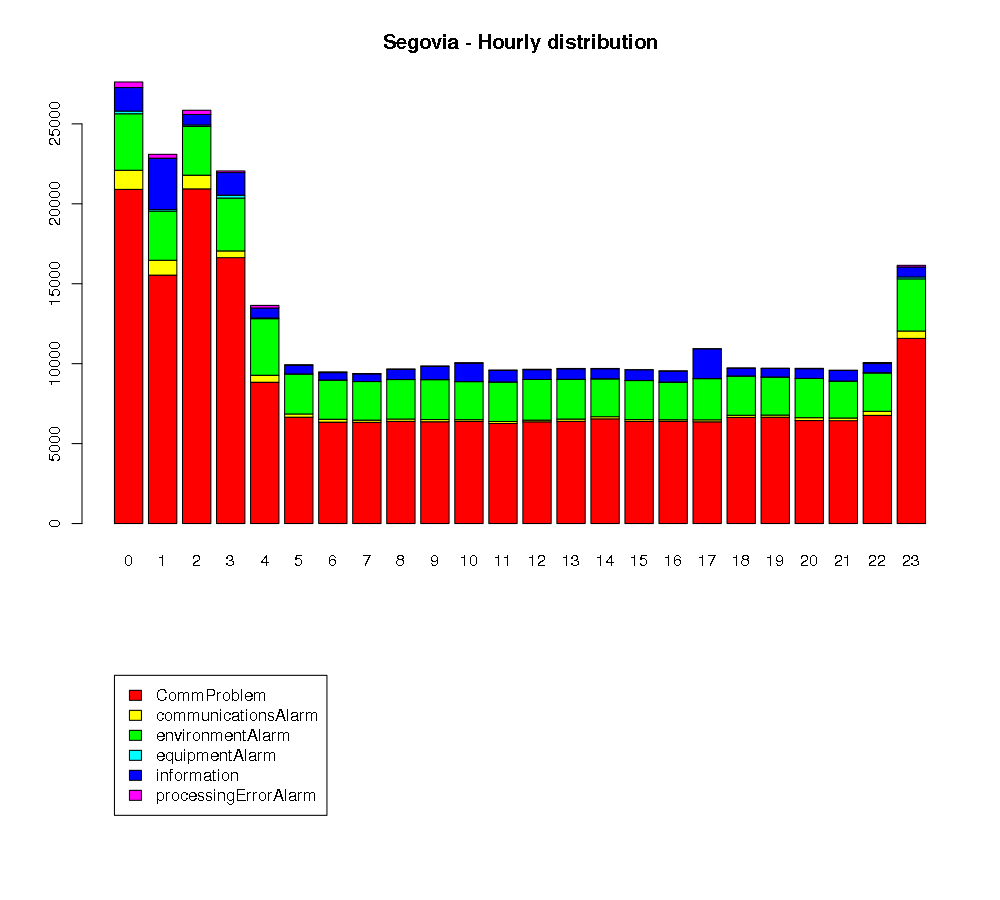
\includegraphics[height=0.4\textheight]{./img/segovia_timeline.png}
 \caption{Hourly distribution for Segovia (stacked)}
\end{figure}
\begin{figure}[h!]
 \centering
 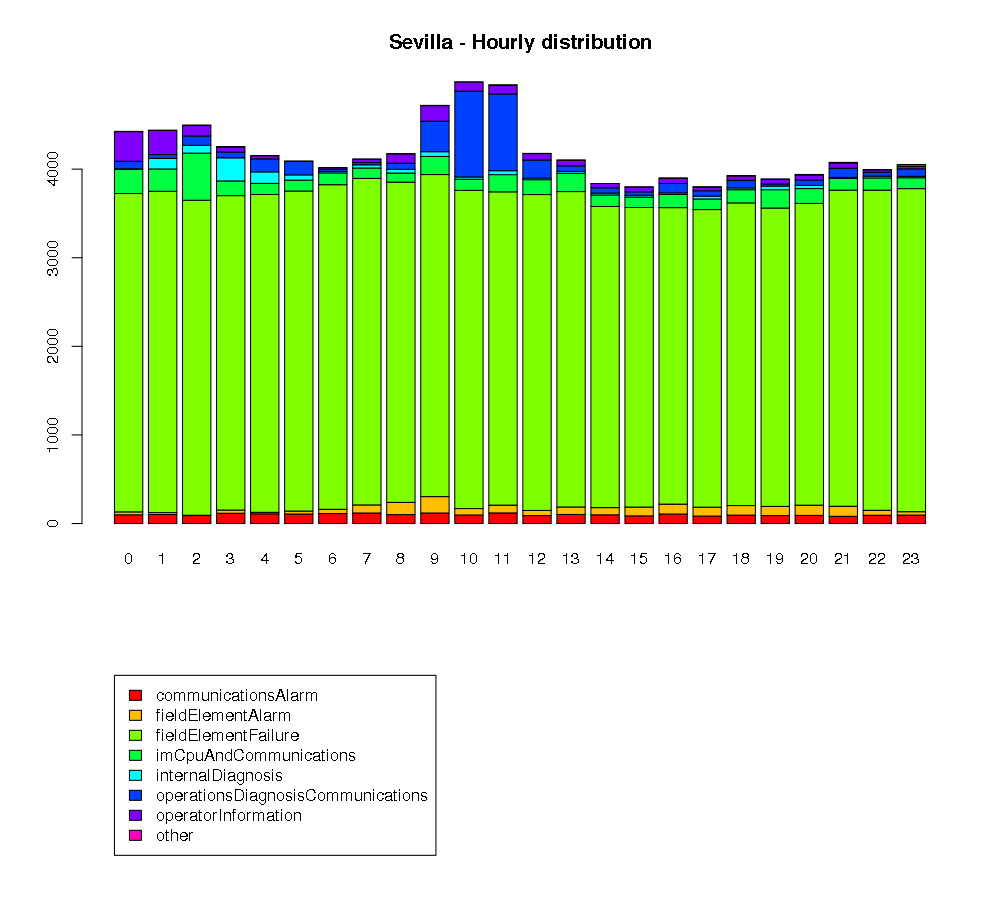
\includegraphics[height=0.4\textheight]{./img/sevilla_timeline.png}
 \caption{Hourly distribution for Sevilla (stacked)}
\end{figure}

\clearpage

\subsubsection{Daily correlation}

We have also generated graphics for correlation between number of alarms of each type during the day, and occurrences of other types of alarms. The result is as follows:

\begin{figure}[h!]
 \centering
 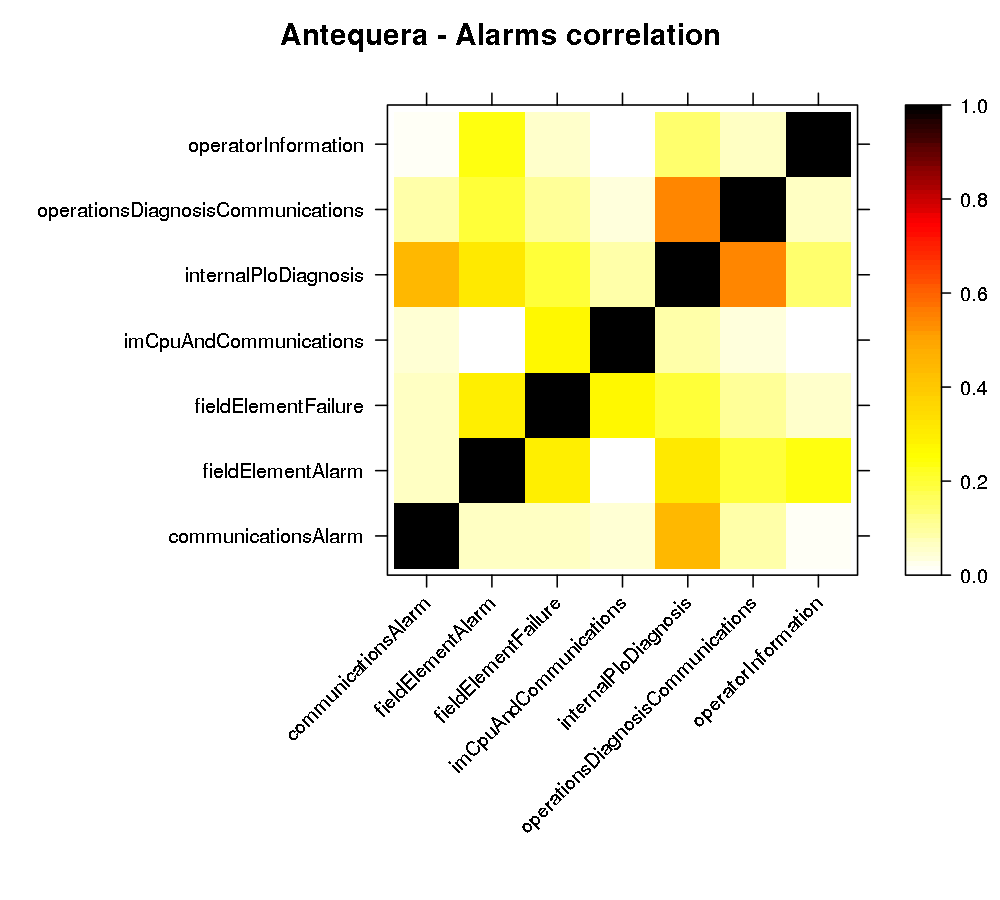
\includegraphics[height=0.4\textheight]{./img/antequera_corr.png}
 \caption{Daily correlation for Antequera}
 \label{fig:anteq_corr}
\end{figure}
\begin{figure}[h!]
 \centering
 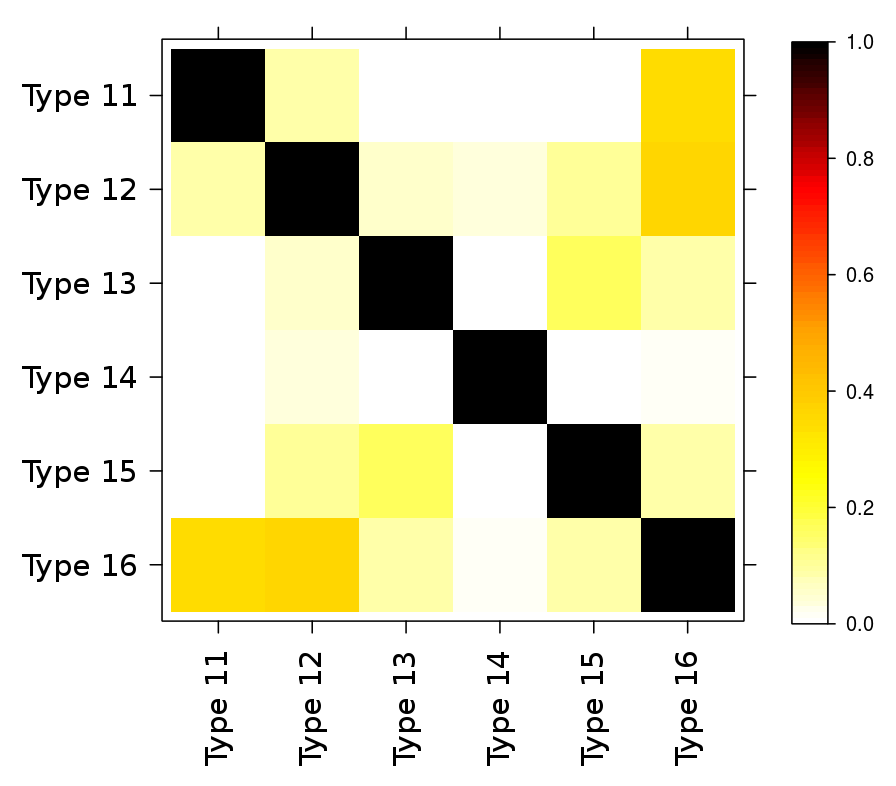
\includegraphics[height=0.4\textheight]{./img/segovia_corr.png}
 \caption{Daily correlation for Segovia}
 \label{fig:segovia_corr}
\end{figure}
\begin{figure}[h!]
 \centering
 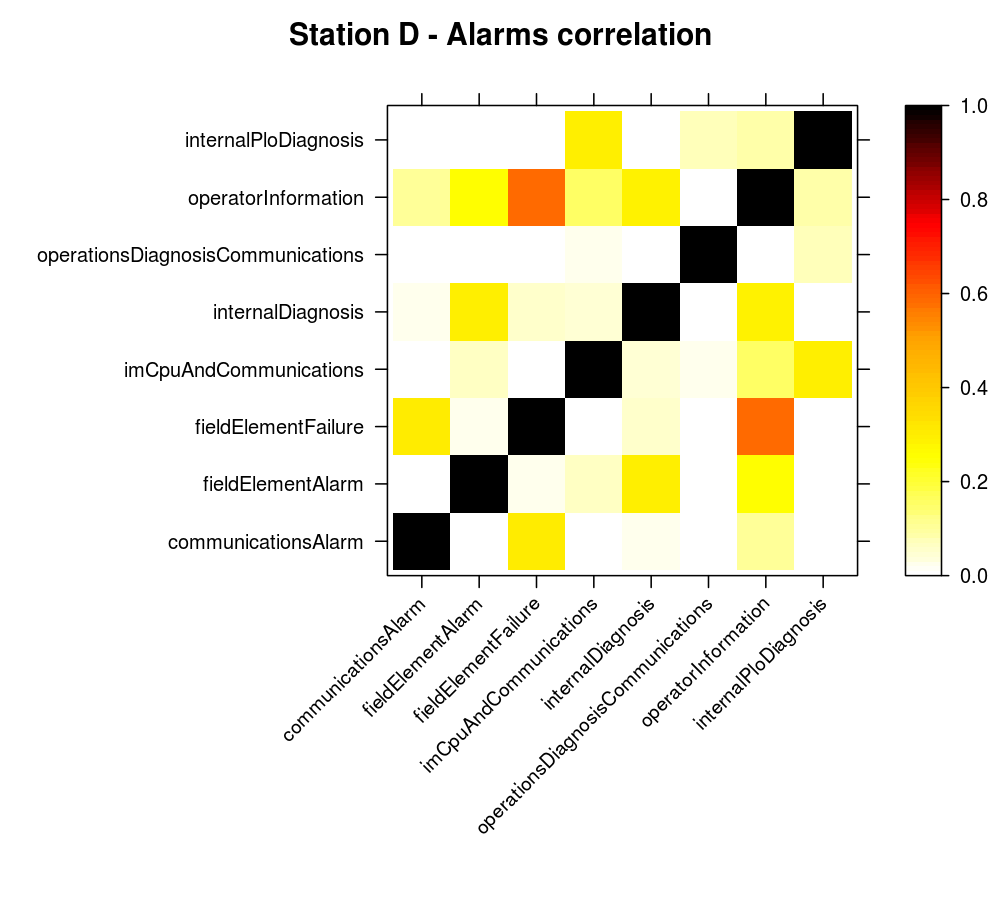
\includegraphics[height=0.4\textheight]{./img/sevilla_corr.png}
 \caption{Daily correlation for Sevilla}
 \label{fig:sevilla_corr}
\end{figure}

\clearpage


\bibliographystyle{plain} 
\bibliography{datamining}

\end{document}


